\chapter{General Concept}
\label{General:2.0}
For a better understanding of the implementation of 6LoWPAN, some general concepts and background knowledge needs to be reviewed. This chapter will give a brief introduction of WSNs, follow by IEEE 802.15.4 and IPv6.

\section{Wireless Sensor Networks}
\label{General:WSN}

As the name implies, WSNs are wireless networks formed by sensor
nodes (also known as motes)\@. A WSN is a typical and important example of a Wireless Personal
Area Network (WPAN)\@. Since technology is continually advancing, and along with the rapid growth of Internet, it can be easily projected that in the not very far future WSNs can be used in nearly all everyday objects to form the ``real'' Internet of Things. In the meantime, however, due to the physical properties and limitations of sensors, there are several concerns of forming such WSNs. These include:

\begin{itemize}
\item Memory size - a sensor is typically designed to be small, with very limited memory
size. While technological advancements are always improving, it is none the less far off in the future when a tiny sensor will be able to house enough memory to perform all the functions a user wants it to. Because of this memory constraint, the operation system and the coding method need to be chosen accordingly - it must be quickly accessible, and light-weighted so it fits into the limited memory of a sensor.
\newline

\item Power consumption - sensors which are deployed in WSNs are expected to have a long battery life.  One can quickly agree that power consumption will be of primary importance to sensors placed in remote or hard to access locations.
\newline

\item Cost - sensors should be very low cost if they are to be used in large scale deployments.  For practical and large scale use, the lower the costs the more objects can be fitted with sensors.
\newline

\item  Unattended operation - being able to interact with sensor nodes without being physically
present is very important and necessary.  This means sensors need to be controlled remotely. 
\end{itemize}

\subsection{System Architecture}
\label{General:WSN:SysArc}

Figure~\ref{fig:WSNArc} shows the typical system architecture of a WSN. Each of the sensor nodes supports wireless routing algorithm in the WSN sub-network. Together, they form a multi-hop network via wireless communication. The entire WSN is further connected to the Internet via a gateway node which acts as a protocol translator. Traditionally, this gateway node has to convert the non-standard communication protocols into a language which other devices and sensors in the network understand. Through the gateway, end users can interact with sensor nodes remotely from the Internet. As such, the gateway device holds considerable complexity in its design and deployment. A more sophisticated solution is proposed by IETF, that is, using IEEE 802.15.4 as physical and MAC layer protocol, and IPv6 as network layer protocol. 
\begin{figure}[htbp]
  \begin{center}
    \leavevmode
      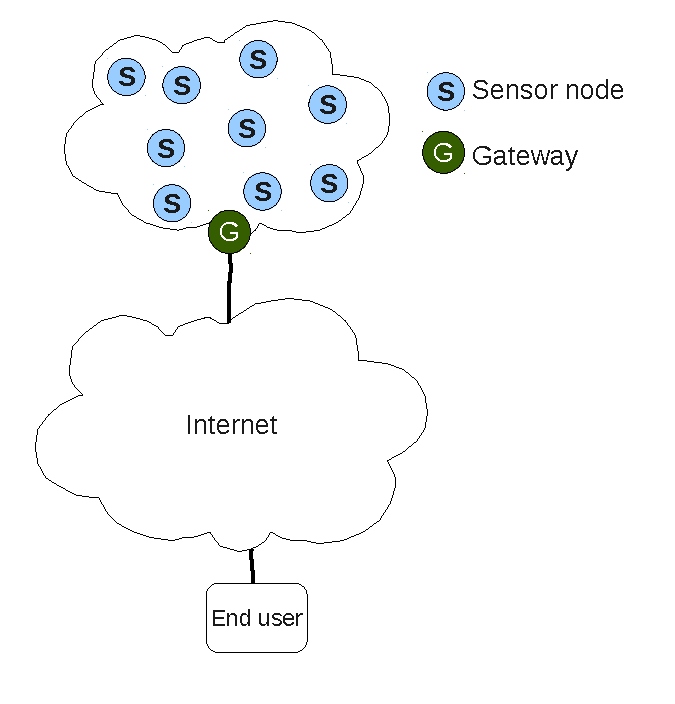
\includegraphics[scale=0.5]
      {/home/bo/Documents/Thesis/Final/Template/Pics/WSNArc.pdf}
   \caption{System architecture for WSN}
    \label{fig:WSNArc}
  \end{center}
\end{figure}

\subsection{The Lower Layers Standard - IEEE 802.15.4}
\label{General:WSN:IEEE}
The physical layer of IEEE 802.15.4 is in charge of data transmission and reception in the physical medium, as well as channel selection and energy management. It operates mainly on three frequency bands: 868-868.6 MHz band for Europe, 902-928 MHz for North America and 2400-2483.5 MHz worldwide. The maximum Service Data Unit (SDU) size that the physical layer is able to receive is 127 octets. 
\newline

Functions of the IEEE 802.15.4 Media Access Control (MAC) layer are: beacon management, channel access, guaranteed time slot management, and data transfer service for upper layers. According to IEEE 802.15.4 definition it can use a 64-bit unique identifier, or a short 16-bit identifier. There are four kinds of frame structures: beacon frame, data frame, acknowledgement frame and MAC command frame. More detailed information about IEEE 802.15.4 can be found in~\cite{IEEE 802.15.4}.
\newline

IEEE 802.15.4 provides wireless communication with short-range, low data-rate communication, low memory requirement, and appropriate power management by defining the physical layer and MAC sub-layer for a low-rate WPAN (LR-WPAN)\@. All these features make IEEE 802.15.4 a promising lower layer protocol for WSNs. 

\subsection{The Network Layer - IPv6}
\label{General:WSN:IPv6}

Being the most accepted network layer protocol, the IP protocol mainly features a universal narrow waist which hides the underlying link technology from the upper layer applications. The traditional IPv4 provides for at most $2^3^2$ addresses. However, judging by the speed of Internet growth, it was predicted that all IP address would soon be exhausted. On July 25, 1994, the IETF proposed IPv6 with $2^1^2^8$ addresses to be the next generation protocol~\cite{RFC 1752}.
\newline

By implementing IPv6, WSNs can communicate directly with other IP based networks and nodes without intermediate entities. The architecture of a WSN with IPv6 applied is shown in Figure~\ref{fig:Ipv6WSNArc}.
\begin{figure}[htbp]
  \begin{center}
    \leavevmode
      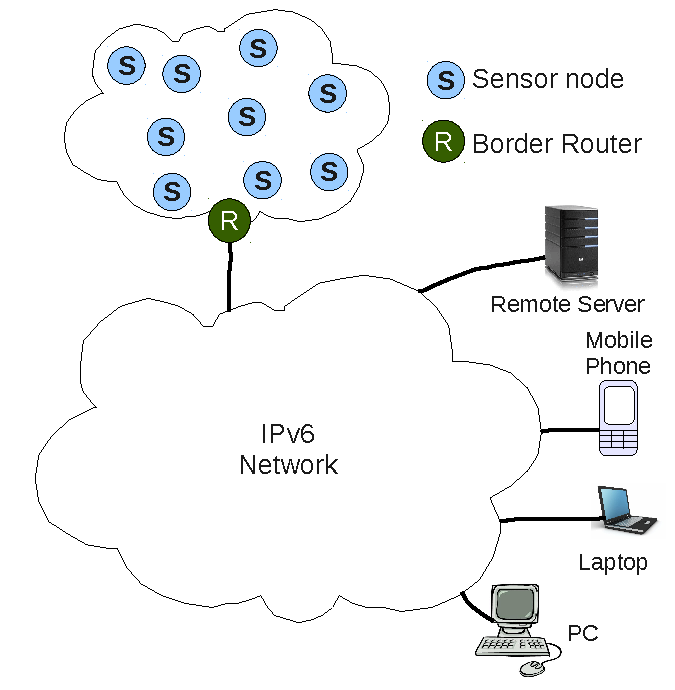
\includegraphics[scale=0.4]
      {/home/bo/Documents/Thesis/Final/Template/Pics/Ipv6WSNArc.pdf}
   \caption{System architecture for WSN with IPv6}
    \label{fig:Ipv6WSNArc}
  \end{center}
\end{figure}
\index{figure 2.2}

Compared with  Figure~\ref{fig:WSNArc}, an IPv6 implemented WSN uses a Border Router (BR) instead of a gateway  to connect the network to the Internet. This kind of network layer router is much more efficient and easier to design than a protocol translating gateway as it eliminates the need for superfluous translations between potentially large number of protocols, which impairs the entire system's usability and usefulness. Furthermore, the 6LoWPAN network can be connected to any other IP based device, giving it extreme adaptability and flexibility unmatched in traditional gateway systems. 
\newline

More advantages of using IPv6 include (but are not limited to):  
\begin{itemize}
\item IP networks are ubiquitous and pervasive in the current society.  This allows for a use of already completed infrastructures, thus saving time, money and R\&D on building new communication platforms.
\newline
 
\item Technologies which use IP are thoroughly researched and known to be safe and reliable.  This saves much effort which would need to be spent in testing and debugging new networking technologies. 
\newline

\item Another reason why IP technologies might prove more suitable are because much of the intellectual rights held by companies in this field are easily traded and used by many players in the field, as opposed to potential lawsuits and legal hassle which might arise due to large-scale usage of new technologies whose intellectual property rights might not be as transparent as the current IP based ones.
\newline

\end{itemize}

As mentioned in Section~\ref{General:WSN:IEEE}, the maximum SDU size that the IEEE 802.15.4 physical layer is able to receive is 127 octets. In the worst-case scenario, this will leave only 81 octets for the MAC layer frame. Meanwhile, IPv6 takes 1280 octets as its Maximum Transmission Unit (MTU) \cite{RFC 4919}. How to fit this 1280 octets IP datagram into a much smaller MAC frame was one of the big concerns. To solve the  size incompatibility and other problems brought by integration of IPv6 and WSN, IETF proposed a series of standards which will be presented in the next charpter.

%}}}

%{{{ Emacs Local Variables

% Local Variables: 
% mode: latex
% TeX-master: "studentprojectthesis"
% TeX-command-list: (("TeX" "tex '\\nonstopmode\\input %t'" TeX-run-TeX nil t) ("TeX Interactive" "tex %t" TeX-run-interactive nil t) ("LaTeX" "%l '\\nonstopmode\\input{%t}'" TeX-run-LaTeX nil t) ("LaTeX Interactive" "%l %t" TeX-run-interactive nil t) ("LaTeX2e" "latex2e '\\nonstopmode\\input{%t}'" TeX-run-LaTeX nil t) ("SliTeX" "slitex '\\nonstopmode\\input{%t}'" TeX-run-LaTeX nil t) ("View" "%v " TeX-run-background t nil) ("Print" "%p " TeX-run-command t nil) ("Queue" "%q" TeX-run-background nil nil) ("File" "dvips %d -o %f " TeX-run-command t nil) ("BibTeX" "bibtex %s" TeX-run-BibTeX nil nil) ("Index" "makeindex -s indexeng.ist %s" TeX-run-command nil t) ("Check" "lacheck %s" TeX-run-compile nil t) ("Spell" "<ignored>" TeX-run-ispell nil nil) ("Other" "" TeX-run-command t t) ("Makeinfo" "makeinfo %t" TeX-run-compile nil t) ("AmSTeX" "amstex '\\nonstopmode\\input %t'" TeX-run-TeX nil t) ("GloTeX" "glotex %t" TeX-run-command nil nil))
% folded-file: t
% End: 

%}}}
